W raporcie opisujemy jedynie te tabele, które zostały utworzone bezpośrednio przez nas, ponieważ baza danych zawiera dodatkowo tabele, które tworzone są przez Django w momencie inicjalizacji projektu.
Poniżej zamieszczony został diagram przedstawiający tabele i relacje między nimi:
\begin{figure}[H]
\centering
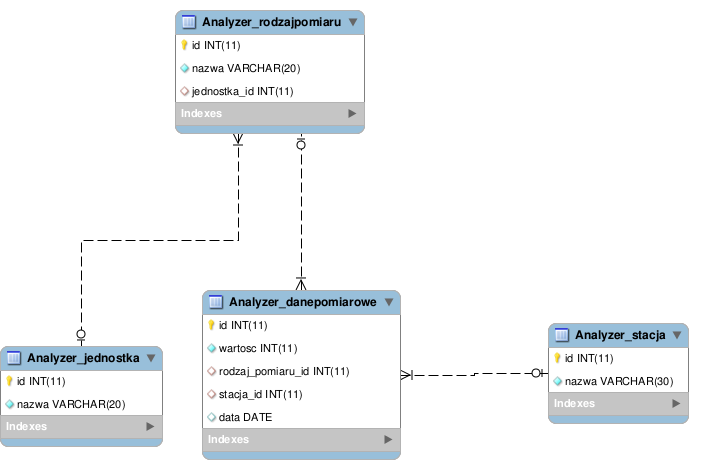
\includegraphics[width=\linewidth]{diagramEER}
\caption{Diagram tabel}
\label{fig:diagramTabel}
\end{figure}

 Poniższa tabela zawiera pełne zestawienie pól stworzonych tabel.
\begin{longtable}{|p{0.25\linewidth}|p{0.25\linewidth}||p{0.5\linewidth}|}
\hline
\textbf{Nazwa tabeli} & \textbf{Nazwa pola} & \textbf{Opis pola} \tabularnewline \hline \hline
\multirow{5}{*}{Analyzer\_danepomiarowe} & id & klucz główny (automatycznie inkrementowany) \tabularnewline\cline{2-3}
 & wartosc & całkowita część danej pomiarowej \tabularnewline\cline{2-3}
 & rodzaj\_pomiaru\_id & klucz obcy \tabularnewline\cline{2-3}
 & stacja\_id & klucz obcy \tabularnewline\cline{2-3}
 & data & data (godzina jest ignorowana) \tabularnewline\hline
\multirow{2}{*}{Analyzer\_jednostka} 
 & id & klucz główny (automatycznie inkrementowany) \tabularnewline\cline{2-3}
 & nazwa & jednostka pomiaru (np. C lub F dla temperatury) \tabularnewline\hline
\multirow{3}{*}{Analyzer\_rodzajpomiaru}
 & id & klucz główny (automatycznie inkrementowany) \tabularnewline\cline{2-3}
 & nazwa & nazwa rodzaju pomiaru, która będzie wykorzystywana do wyboru danych pomiarowych w aplikacji internetowej \tabularnewline\cline{2-3}
 & jednostka\_id & klucz obcy \tabularnewline\hline
\multirow{2}{*}{Analyzer\_stacja}
 & id & klucz główny (automatycznie inkrementowany) \tabularnewline\cline{2-3}
 & nazwa & nazwa stacji, która będzie wykorzystywana do wyboru danych pomiarowych w aplikacji internetowej \tabularnewline\hline
\end{longtable}

